\documentclass{sig-alt-hotnets}

\usepackage{times}
\usepackage{xcolor}
\usepackage{xspace}
\usepackage{boxedminipage}
\usepackage{pifont}
\usepackage{fancyvrb}
\usepackage{wrapfig}
\usepackage{pseudocode}
\usepackage{outlines}
\usepackage[sort]{cite}

\definecolor{MyDarkBlue}{rgb}{0,0.08,0.45}
\usepackage[pdftex]{hyperref}
\hypersetup{
  colorlinks,%
  citecolor=MyDarkBlue,%
  filecolor=MyDarkBlue,%
  linkcolor=MyDarkBlue,%
  urlcolor=MyDarkBlue
}
\usepackage{fixltx2e}
\usepackage{textgreek}

\newcommand{\projectname}{{STS}}
\newcommand{\projectmeaning}{the SDN Troubleshooting Simulator}
\newcommand{\simulator}{retrospective causal inference}
\newcommand{\Simulator}{Retrospective causal inference}
\newcommand{\SIMULATOR}{RETROSPECTIVE CAUSAL INFERENCE}

\newcommand{\tbd}[1]{{\bf [[TBD: {#1}]]}}
\newcommand{\ie}{{\it i.e.}}
\newcommand{\eg}{{\it e.g.}}
\newcommand{\cf}{{\it cf.}}
\newcommand{\etc}{{\it etc.}}
\newcommand{\viz}{{\it viz.}}
\newcommand{\apriori}{{\it a priori}}
\newcommand{\eat}[1]{}

\newcommand{\teemu}[1]{{\color{ForestGreen}\bf TK: {#1}}}
\newcommand{\scott}[1]{{\color{purple}\bf SS: {#1}}}
\newcommand{\andi}[1]{{\color{blue}\bf AW: {#1}}}
\newcommand{\andrew}[1]{{\color{BrickRed}\bf SW: {#1}}}
\newcommand{\sam}[1]{{\color{orange}\bf SW: {#1}}}
\newcommand{\colin}[1]{{\color{red}\bf CS: {#1}}}

%\newcommand{\teemu}[1]{}
%\newcommand{\scott}[1]{}
%\newcommand{\andi}[1]{}
%\newcommand{\andrew}[1]{}
%\newcommand{\sam}[1]{}
%\newcommand{\colin}[1]{}

% Notes:
\newcommand{\num}[1]{{\color{red}\bf {#1}}}

% Delta-debugging symbols:
\newcommand{\PASS}{\text{\ding{52}}\xspace}
\newcommand{\DFAIL}{\text{\ding{56}}\xspace}
\newcommand{\cpass}{{T_{\scriptscriptstyle \PASS}}}
\newcommand{\cfail}{{T_{\scriptscriptstyle \DFAIL}}}
\newcommand{\dpass}{{T'_{\scriptscriptstyle \PASS}}}
\newcommand{\dfail}{{T'_{\scriptscriptstyle \DFAIL}}}
\newcommand{\done}{{T_{\scriptscriptstyle 1}}}
\newcommand{\dtwo}{{T_{\scriptscriptstyle 2}}}
\newcommand{\test}{\textit{replay}\xspace}
\newcommand{\ddmin}{\textit{ddmin}\xspace}

\sloppy
\begin{document}
    \date{}

\title{How Did We Get Into This Mess?}
\subtitle{Isolating Fault-Inducing Inputs to SDN Control Software}

\author{Paper \#15}

\date{}
    \maketitle
    \thispagestyle{empty}

\abstract{{\it The predominant technique for troubleshooting bugs in software-defined networks,
log analysis, is tedious and error-prone. We argue that a more principled
approach should be built around identifying inconsistencies between lower-level
network configuration and higher-level policies dictated by control
applications. Towards this end we present
cross-layer correspondence checking, a mechanism to automatically detect and
isolate inconsistencies due to bugs in the SDN platform. In
eventually-consistent systems such as SDN however,
transient inconsistencies between policy and configuration are inevitable.
We therefore augment correspondence checking with \simulator{} to help troubleshooters
distinguish pernicious persistent from harmless ephemeral inconsistencies. We
show that these techniques combine to help troubleshooters ``see through the fog'' of
diagnostic information.
}}

\section{Introduction}
\label{sec:intro}
The SDN platform's $raison\text{ }d'\hat{e}tre$ is to 
hide complexity from control applications. Modern controllers perform
replication, resource arbitration, failure recovery, and network 
virtualization on the control application's behalf. 

Despite the abstractions provided by the SDN programming model,
software-defined networks are no less complex than traditional networks. The architectural goal of SDN is
simply to push complexity from the control application onto the underlying platform.

SDN control platforms are prone to bugs as a result of their complexity. Bugs in the
platform present an architectural tension: troubleshooting requires
access to precisely the same details hidden by the platform's abstractions.
When an application developer 
encounters erratic behavior in the network, they must trace their
policy specification through multiple layers of abstraction
preceding changes in the physical network: virtualization logic,
distribution logic, and network devices. The error's root cause
may manifest in any of these layers, not just the control application.

As it stands, the SDN platform provides meager support for troubleshooting.
The predominant troubleshooting method is log analysis: manually
specifying log statements at relevent points throughout the system,
collecting, gathering, and ordering distributed log files, and analyzing the
results {\it post-hoc} when a error is encountered in production. Besides its
apparent tediousness, this approach is lacking in several ways: logs events
are enormous in number, impossible to aggregate into a single serial
execution of the system, and often at the wrong level of granularity to be of
use. \colin{</ why it's hard>}

Recent work has contributed much-needed improvements to this state of affairs. 
NICE applies concolic execution and model checking to SDN control
applications, thereby automating testing and catching bugs before
they are deployed~\cite{nice}. Aneater~\cite{anteater} and HSA~\cite{hsa}
introduce mechanisms for checking static invariants in the dataplane.
Nevertheless, no troubleshooting mechanism exists yet for the SDN platform itself.

New operating system abstractions face an arduous path towards adoption
without sound troubleshooting mechanisms. Analogously, the success of the
SDN programming model depends heavily on the utility of its troubleshooting
paradigm. Our goal in this paper is to work towards a useful
troubleshooting mechanism for the SDN platform. \colin{</ why it's important>}

We observe that in eventually-consistent systems such as sofware-defined networks,
transient inconsistencies are an inevitable property of the system.
Consequently, the process of troubleshooting errors essentially boils down to
identifying relevant events amongst a clamor of inconsistencies and diagnostic
information.

We present two mechanisms designed to make it easier for operators and
developers to ``see through the noise'' of diagnostic information. The first,
cross-layer correspondence checking, leverages the structure of the SDN
architecture to enable a general and verifiable notion of platform
correctness. Correspondence checking allows troubleshooters to isolate the cause of 
an inconsistency to a particular layer without needing to define invariants or
instrument third-party code. Our second
mechanism, simulated replay analysis, allows troubleshooters 
to differentiating ephemeral from persisent inconsistencies by steering the
execution of the system forward and backward in time, filtering out extraneous
external events, and inducing uncommon events such as failures. \colin{</ what we did>}

The rest of this paper is organized as follows. In \S\ref{sec:overview},
we present an overview of the SDN stack and its failure modes.
In \S\ref{sec:approach} we present correspondence checking and simulated
replay analysis in detail. In \S\ref{sec:evaluation} we present
two use-cases of our techniques, as well as a preliminary evaluation
of their runtime. Finally, in \S\ref{sec:related_work} we discuss related work,
and in \S\ref{sec:conclusion} we conclude.


\section{Minimal Causal Sequences}
\label{sec:formalism}
We represent the forwarding state of the network
at a particular time as a configuration $C$.
An invariant is a predicate $P$ over forwarding state (a safety
condition). We say that forwarding
state $C$ violates an invariant if $P(C)$ does not
hold, also denoted as $\overline{P}(C)$.

Log $L$ consists of external events $E_L$ and observed internal events $I_L$,
along with a timing $T_L$ of the observed events.
We assume that all changes to forwarding state can be inferred
from internal events (\eg~OpenFlow message sends), so
that at all times we have knowledge of the relevant forwarding state.
Therefore we can determine from $L$ whether $P$ failed to hold at any point.
% It might make the notation more concise if we just include the sequence of
% forwarding configurations as part of L. We have access to this information
% in practice, since we're driving the fuzzing.

A replay of a log means replaying the external events along with a particular timing (or interleaving) $T$.
We denote this by $replay(E_L,T)$.
The output of $replay$ is a sequence of forwarding state configurations
$C_1,C_2,\dots,C_n$.
We say that a replay reproduces an invariant violation if
$\exists_{C_i \in replay(E,T)}\:s.t.\:\overline{P}(C_i)$.
In the ideal case $replay(E_L,T_L)$ reproduces the orignal invariant violation
asociated with $L$ (as long as there is no nondeterminism). \\

\noindent~Troubleshooting process:

\begin{outline}
\1 Start with log $L$ where $P$ did not hold at some point. Could be operational or fuzzed log.

\1 Definition: an MCS is a subsequence $E_M$ of $E_L$ and a timing $T_M$ such
that $replay(E_M,T_M)$ reproduces the invariant violation, but for all proper
subsets $E_L$ of $E_M$
there is no timing $T$ s.t. $replay(E_L,T)$ reproduces the violation.

\1 Assumption 1: naturally occurring external logs $E_L$ are large.

\1 Assumption 2: the MCS of most natural logs resulting in violations are much smaller than the original log.  That is, bugs are causally sparse.
\end{outline}

\noindent~Technical challenge: Find approximations to MCSs.

\begin{outline}
\1 Dumb approach: explore all timings $T$ for each subset $E$.

\1 Slightly smarter approach: use delta debugging, causality, and equivalence to limit set of timings $T$ you need to look at.
\end{outline}


\section{Approach}
\label{sec:approach}
Given a log $(E_L, T_L, C_L)$ generated from testing infrastructure exhibiting an invariant violation,
our goal is to identify its MCS. This involves two tasks:
searching through subsequences of $E_L$, and searching for replay timings for those
subsequences that, if possible, trigger the original invariant violation.

\eat{
We introduce our approach using an example bug in the Floodlight open-source control
platform~\cite{floodlight_bug}. Floodlight is distributed across
multiple controllers for high availability, and provides support for
virtualization. Switches maintain one hot connection to a master controller and
several cold connections to replica controllers. The \emph{master} holds the
authority to modify the configuration of switches, while the other
controllers are in \emph{backup} mode and do not change the
switch configurations unless they detect that the master has crashed.

\begin{figure}[t]
  %\hspace{-10pt}
  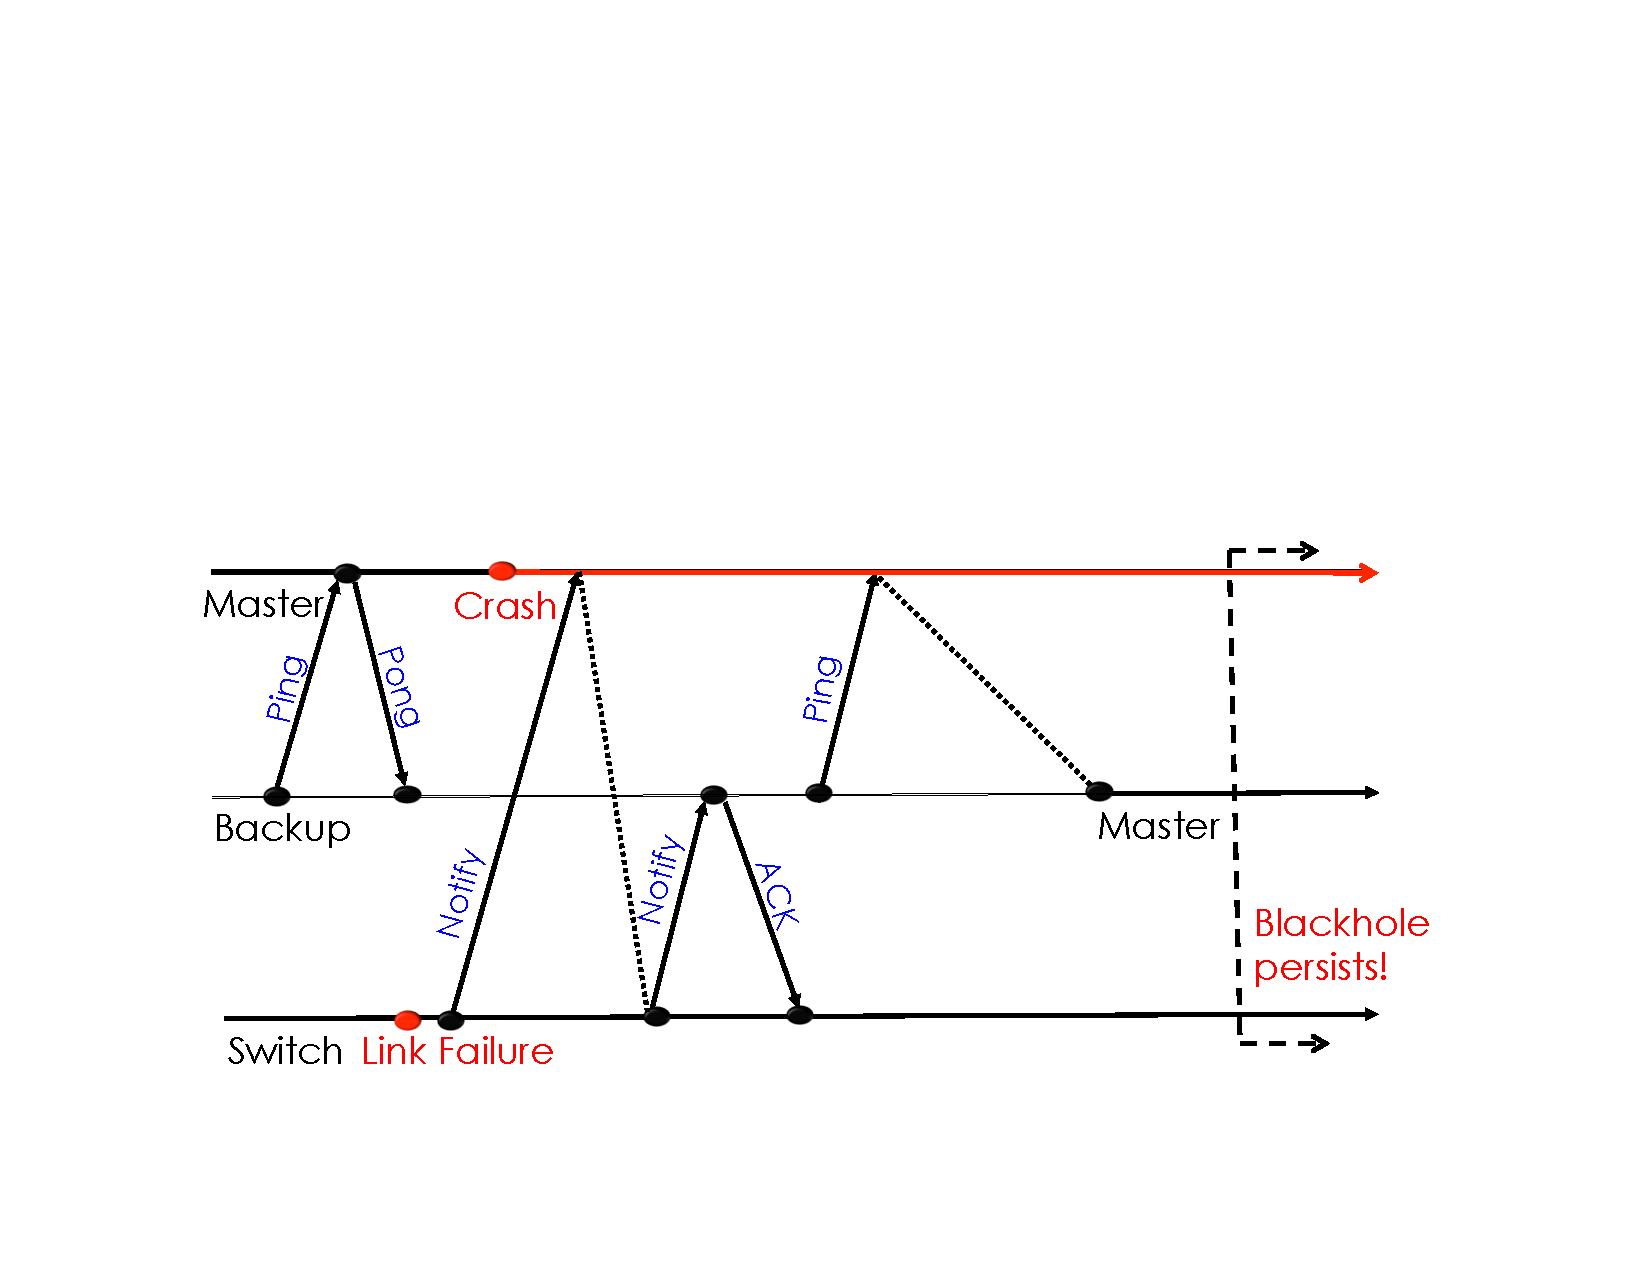
\includegraphics[width=3.25in]{../diagrams/case_study/example_bug.pdf}
  \caption[]{\label{fig:example} Floodlight failover bug. External inputs
             are depicted as red dots, internal events are depicted as black
             dots, and the dotted message line depicts a timeout.}
\end{figure}

The failover logic in Floodlight is incorrect, leading to the
following race condition\footnote{Note that this issue was
originally documented by the developers of Floodlight~\cite{floodlight_bug}.} depicted in
Figure~\ref{fig:example}:
a link fails (E1), and the switch attempts to notify the controllers (E2,E4) shortly after the master
controller has died (E3), but before a new master has been selected (E6). In this case, all live controllers are in
the backup role and will not take responsibility for updating the switch
flow table (E5). At some point, a backup notices the master failure and
elevates itself to the master role (E6). The new master will proceed to manage
the switch, but without ever clearing the routing entries for
the failed link, resulting in a persistent blackhole. In this example, the MCS
is the conjunction of the two external inputs (E1,E3).
}

\subsection{Searching for Subsequences}
\label{subsec:delta_debugging}

Checking random subsequences of $E_L$ would be one viable but inefficient
approach to achieving our first task. We do better by leveraging
%divide-and-conquer search technique from the software engineering community:
the delta debugging algorithm~\cite{Zeller:1999:YMP:318773.318946}, a
divide-and-conquer algorithm for
isolating fault-inducing inputs. In our case, we use delta
debugging to iteratively select subsequences of $E_L$ and replay each
subsequence with some timing $T$. If the bug persists for a given subsequence, delta debugging ignores the
other inputs, and proceeds with the search for an MCS within this subsequence.
%In what follows, we use the term {\em delta debugging} to refer to our algorithm for finding relevant subsequences.
The delta debugging algorithm is shown in Figure~\ref{fig:ddmin}.
%(with `$test$' replaced by `$replay$').

The input subsequences chosen by delta debugging are not always
valid. Of the possible inputs sequences we generate (shown in
Table~\ref{tab:inputs}), it is not sensible to replay a recovery event without a
preceding failure event, nor to replay a host migration
event without modifying its starting position when a preceding host
migration event has been pruned. Our implementation of delta debugging
therefore prunes failure/recovery event pairs as a single unit, and updates initial host locations
whenever host migration events are pruned so that hosts do not magically appear at new
locations.\footnote{Handling invalid inputs is crucial for
ensuring that the delta debugging algorithm finds a minimal causal
subsequence. The algorithm we employ~\cite{Zeller:1999:YMP:318773.318946}
makes three
assumptions about inputs: monotonicity, unambiguity, and consistency.
An event trace that violates monotonicity may contain events that ``undo'' the
invariant violation triggered by the MCS, and may therefore exhibit slightly
inflated MCSes. An event trace that violates unambiguity may exhibit multiple MCSes; delta debugging
will return one of them. The most important assumption is consistency, which
requires that the test outcome can always be determined.
We guarantee neither monotonicity nor unambiguity, but we guarantee consistency by
ensuring that subsequences are always semantically valid by applying the two
heuristics described above. Zeller wrote a follow-on
paper~\cite{Zeller:2002:SIF:506201.506206} that removes the need for these
assumptions, but incurs an additional factor of $n$ in complexity in doing so.}
These two heuristics account for validity of all network
events shown in Table~\ref{tab:inputs}. We do not yet
support network policy changes as events, which have more complex semantic
dependencies.\footnote{If codifying the semantic dependencies of
policy changes turns out to be difficult, one could just employ the more
expensive version of delta debugging to account for
inconsistency~\cite{Zeller:2002:SIF:506201.506206}.}

\begin{figure*}[t]
\begin{boxedminipage}{\textwidth}
Input: $\cfail$ s.t. $\cfail$ is a trace and $\test(\cfail) = \DFAIL$. Output: $\dfail
= \ddmin(\cfail)$ s.t. $\dfail \subseteq
\cfail$, $\test(\dfail) = \DFAIL$, and~$\dfail$ is minimal.
\begin{align*}
\ddmin(\cfail) &= \ddmin_2(\cfail, \emptyset) \quad \text{where} \\
\ddmin_2(\dfail, R) &=
\begin{cases}
\dfail & \text{\hphantom{else }if $|\dfail| = 1$ (``base case'')} \\
\ddmin_2\bigl(\done, R\bigr) &
\text{else if $\test(\done \cup R) = \DFAIL$ (``in $\done$'')} \\
\ddmin_2\bigl(\dtwo, R\bigr) &
\text{else if $\test(\dtwo \cup R) = \DFAIL$ (``in $\dtwo$'')} \\
\ddmin_2\bigl(\done, \dtwo \cup R\bigr) \cup \ddmin_2\bigl(\dtwo, \done \cup
R\bigr) & \text{otherwise (``interference'')}
\end{cases}
\end{align*}
\begin{center}
where $\test(T)$ denotes the state of the system after executing the trace $T$,
$\DFAIL$ denotes a correctness violation, \\
$\done \subset \dfail$, $\dtwo \subset \dfail$, $\done \cup \dtwo = \dfail$, $\done \cap
\dtwo = \emptyset$, and $|\done| \approx |\dtwo| \approx |\dfail| / 2$
hold.
\end{center}
\end{boxedminipage}
\caption{\colin{Cut if we need space} Automated Delta Debugging Algorithm From~\cite{Zeller:1999:YMP:318773.318946}}
\label{fig:ddmin}
\end{figure*}

\eat{ % Original O(n^2) algorithm
\begin{figure*}[t]
\caption{Minimizing Delta Debugging Algorithm From~\cite{Zeller:2002:SIF:506201.506206}}
\begin{boxedminipage}{\textwidth}
Input: $\cfail$ s.t. $\cfail$ is a trace and $\test(\cfail) = \FAIL$. Output: $\dfail
= \ddmin(\cfail)$ s.t. $\dfail \subseteq
\cfail$, $\test(\dfail) = \FAIL$, and~$\dfail$ is 1-minimal.
\begin{align*}
\ddmin(\cfail) &= \ddmin_2(\cfail, 2) \quad \text{where} \\
\ddmin_2(\dfail, n) &= 
\begin{cases}
\ddmin_2(\Delta_i, 2) & \text{\hphantom{else }if $\exists i \in \{1, \dots, n\} \cdot \test(\Delta_i) = \FAIL$ (``reduce to subset'')} \\
\ddmin_2\bigl(\nabla_i, \max(n - 1, 2)\bigr) & 
\text{else if $\exists i \in \{1, \dots, n\} \cdot \test(\nabla_i) = \FAIL$ (``reduce to complement'')} \\
\ddmin_2\bigl(\dfail, \min(|\dfail|, 2n)\bigr) & \text{else if $n < |\dfail|$ (``increase granularity'')} \\
\dfail & \text{otherwise (``done'').}
\end{cases}
\end{align*}
where $\test(T)$ denotes the state of the system after executing the trace $T$,
$\FAIL$ denotes a correctness violation, \\
$\nabla_i = \dfail - \Delta_i$, $\dfail = \Delta_1 \cup \Delta_2 \cup \dots \cup \Delta_n$, all
$\Delta_i$ are pairwise disjoint sequences of inputs, and $\forall \Delta_i \cdot |\Delta_i| \approx |\dfail| / n$
holds.
\end{boxedminipage}
\label{fig:ddmin}
\end{figure*}
}

\subsection{Searching for Timings}
\label{subsec:algorithm}

Simply exploring subsequences of $E_L$ is insufficient for finding MCSes: the
timing of those subsequences in each invocation of $replay()$ is crucial for reliably
reproducing the
invariant violation. The most natural approach would be to maintain the original
timings between the remaining original inputs for each subsequence.
\eat{\ie~if we
define $t_i$ as the timestamp of the $i^{th}$ input from the original run and $t'_i$ as the
replay clock value when it injects that same input
(which may or may not be the $i$'th input in the subsequence), then we might
just set $t'_i = t_i$.
\eat{
\begin{align*}
t'_0 = t_0 \\
t'_i = t'_{i-1} + |t_{i} - t_{i-1}|
\end{align*}
}
}
Unfortunately, this approach does not work in practice because it can violate
causal dependencies from the original execution, due to changes in the behavior
of the control software induced by pruning inputs. %\eat{: when we replay only a
%subsequence of the original inputs, the reaction of the control software
%can change, such that it behaves differently or takes a different amount of
%time to respond to the remaining inputs events.
%In practice we have observed that simply maintaining relative timings can
%result in injecting the remaining inputs too early or late.}
To reliably reproduce the invariant violation
we need to inject an input event $e$ only after all other
events, including internal events triggered by the control software itself,
that precede it in the
happens-before~\cite{Lamport:1978:TCO:359545.359563}
relation ($\{i \mid i \rightarrow e\}$) from the original execution have
occurred~\cite{tel2000introduction}.

Internal events include
(a) message delivery events, either between controllers (\eg~database
synchronization messages) or
between controllers and switches (\eg~OpenFlow commands), and (b) state transitions
within controllers (\eg~a backup node deciding to become master).
We obtain visibility into (a) by having our
\tester~(to be described in \S\ref{sec:systems_challenges}) interpose on all message channels.
We optionally obtain visibility into (b) by instrumenting controller
software with a simple interposition layer (to be described in \S\ref{subsec:mitigating}).
With visibility into internal events and control over input events, the
\tester~records a totally-ordered trace by logging an event only after
all prior events are completed.

%\subsection{Preserving Causality}

Maintaining the happens-before relation from the original trace
(which reproduces the violation) throughout replay of subsequences of the
trace (which may or may not reproduce that
violation) involves three issues: coping with syntactic differences in internal
events across runs,
handling internal events from the original
execution that may not occur after pruning, and dealing with new internal events that were not
observed at all in the original execution.

\eat{
\colin{Somewhat redundant. Maybe wait until use cases.}
While the inputs and original internal events are given to us,
we become aware of new internal events throughout replay by
(i) monitoring
control message receipts between controllers and switches,
and (ii) interposing on the controllers' logging library and notifying the
replayer whenever the control software executes a log statement (which serve to mark relevant state
transitions). Note that to achieve truly deterministic
replay, these log statements would need to
be highly granular, capturing information such as thread scheduling decisions;
we show in \S\ref{subsec:case_studies}
however that pre-existing, course granular log statements are often sufficient to
successfully reproduce bugs.}

%\footnote{We discuss this problem further in
%\S\ref{subsec:domain_knowledge}.}
%Note that the developer must provide enough logging statements
%so that relevant internal state transitions are captured and visible to our
%tool.

\begin{table}[tb]
\centering
\footnotesize
\begin{tabular}{|l|l|}
\hline
Internal message & Masked values \\
\hline
\hline
OpenFlow messages & xac id, cookie, buffer id, stats \\
% port numbers?
\hline
packet\_out/in payload & all values except src, dst, data \\
\hline
Log statements & varargs parameters to printf \\
\hline
\end{tabular}
\caption{Internal messages and their masked values. %The masks serve to
%define equivalence classes.
}
\label{tab:fingerprints}
\vspace{-0.5cm}
\end{table}


{\bf Functional Equivalence. } Internal events may differ syntactically (\eg~sequence numbers
of control packets may all differ) when replaying a subsequence of the original log.
We observe that many internal events are {\em functionally
equivalent}, in the sense that they
have the same effect on the state of the system with respect to triggering the
invariant violation (despite syntactic differences). For example, \emph{flow\_mod}
messages may cause switches to make the same change to their forwarding behavior
even if the transaction ids differ.

We leverage this observation by defining
masks over semantically extraneous fields of
internal events.\footnote{One consequence
of applying masks is that bugs involving masked fields are outside the purview of
our approach.} These masks only need to be specified once, and can later be
applied programmatically to event traces.

We show the fields we mask in Table~\ref{tab:fingerprints}. We consider an
internal event $i'$ observed in the replay
equivalent (in the sense of inheriting all of its happens-before relations) to an internal
event $i$ from the original log if and only if all unmasked fields have the same value
and $i$ occurs between $i'$'s preceding and succeeding inputs in the
happens-before relation.

\begin{table}[tb]
\centering
\footnotesize
\begin{tabular}{|l|l|}
\hline
\textbf{Input Type} & \textbf{Implementation} \\
\hline
\hline
Switch failure/recovery & TCP teardown \\
\hline
Controller failure/recovery & \verb=SIGKILL= \\
\hline
Link failure/recovery & \verb=ofp_port_status= \\
\hline
Controller partition & \verb=iptables= \\
\hline
Dataplane packet injection & Network namespaces \\
\hline
Dataplane packet drop & Dataplane interposition \\
\hline
Dataplane packet delay & Dataplane interposition \\
\hline
Host migration & \verb=ofp_port_status= \\
\hline
Control message delay & Controlplane interposition \\
\hline
Non-deterministic TCAMs & Modified switches \\
\hline
\end{tabular}
\caption{Input types currently supported by \projectname}
\label{tab:inputs}
\end{table}

\eat{
\begin{figure}[t]
    %\hspace{-10pt}
    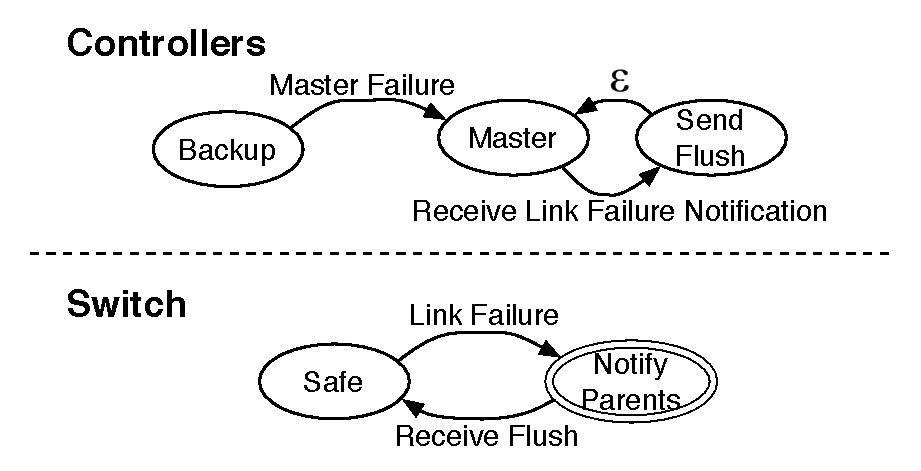
\includegraphics[width=3.25in]{../diagrams/state_machines/controller_switch.pdf}
    \caption[]{\label{fig:state_machines} Simplified state machines for the switch and
    controllers in the example Floodlight bug. Double outlined states
    represent presence of the blackhole.}
\end{figure}
}

{\bf Handling Absent Internal Events. } Some internal events from the original
log which causally ``happen before'' some external input
may be absent when replaying a subsequence of that log.
For instance, if we prune a link failure event, then
the corresponding link failure notification will never arise as an internal event.
\eat{
The control software's state machine (which we do not assume to know) determines whether
internal events cease to appear. Consider the simplified state machines for the switch and
controllers from the Floodlight case shown in
Figure~\ref{fig:state_machines}. If we prune the link failure input, the
master will never receive a link failure notification and
transition to and from \emph{Send Flush}.}

We handle this by attempting to infer the presence of internal
events before we replay each subsequence. Our algorithm (called {\sc Peek()}) for inferring the
presence of internal events is depicted in
Figure~\ref{fig:peek}. The algorithm injects each input, takes a
snapshot\footnote{We discuss the implementation details of snapshotting
in~\ref{subsec:snapshotting}.} of
the network and the control software's state, allows the system to proceed up
until the following input (plus a small time $\epsilon$), records the observed
events, and matches the
recorded events with the functionally equivalent internal events observed in
the original trace. With these inferred causal dependencies, we then replay
the subsequence, this time waiting to inject each input until each of its
(functionally equivalent) predecessors have occurred.\footnote{In the
case that, due
to non-determinism, an internal event occurs during {\sc Peek()} but does not occur
during replay, we time out on internal events after $\epsilon$ seconds of
their expected occurrence.}

\eat{ % Old version without peek()
We handle this possibility by waiting for each expected internal event
for a certain time \textepsilon. If the internal event does not occur within
this time, we assume that it is absent and proceed. If, however, we find
during the \textepsilon~time units we were waiting that another internal that
happens \emph{after} our next input occurs, we know that we have waited too
long and violated causality. In this case we need to restart the replay
process, this time knowing which internal events in the current
input interval are and are not going to occur before injecting the next input.
We show our overall event scheduling algorithm
in Figure~\ref{fig:replay}.
}

\eat{ % Somewhat redundant with peek()
\begin{figure}
  \begin{pseudocode}[framebox]{CausalInference}{events}
    \PROCEDURE{Replay}{subsequence}
    subsequence \GETS \CALL{Peek}{subsequence} \\
    \FOR e\textsubscript{i}\ in\ subsequence \\
      \BEGIN
      \IF e\textsubscript{i}\ is\ an\ internal\ event \\
      \AND e\textsubscript{i}\ is\ not\ marked\ absent:
      \THEN
        \BEGIN
          \Delta \GETS |e\textsubscript{i}.time - e\textsubscript{i-1}.time| + \epsilon \\
          wait\ up\ to\ \Delta\ seconds\ for\ e\textsubscript{i} \\
          \IF e\textsubscript{i}\ did\ not\ occur:
          \THEN mark\ e\textsubscript{i}\ as\ absent
        \END
      \ELSEIF e\textsubscript{i}\ is\ an\ input:
      \THEN
        \BEGIN
          \IF a\ successor\ of\ e\textsubscript{i}\ occurred: \\
          \INLINECOMMENT{waited too long}
          \THEN
            \RETURN{\CALL{Replay}{subsequence}}
          \ELSE
            inject\ e\textsubscript{i}
          \END
        \END
    \ENDPROCEDURE
  \end{pseudocode}
  \caption{{\tt Replay} is responsible for replaying subsequences of events
  chosen by delta debugging and determining
  if the bug reappears. \colin{Fix framebox width.}}
    \label{fig:replay}
\end{figure}
}

\begin{figure}
  \begin{pseudocode}[framebox]{Peek}{events}
    \footnotesize
    \PROCEDURE{Peek}{input\ subsequence}
    inferred \GETS [\ ] \\
    \FOR e\textsubscript{i}\ in\ subsequence \\
    \BEGIN
      snapshot\ system \\
      inject\ e\textsubscript{i} \\
      \Delta \GETS |e\textsubscript{i}.time - e\textsubscript{i-1}.time| + \epsilon \\
      record\ events\ for\ \Delta\ seconds \\
      matched \GETS original\ events\ \&\ recorded\ events \\
      inferred << e\textsubscript{i} << matched \\
      restore\ snapshot \\
    \END \\
    \RETURN{inferred}
    \ENDPROCEDURE
  \end{pseudocode}
  \caption{{\sc Peek} is responsible for determining which internal events
  from the original sequence are going to occur for a given subsequence.
  \label{fig:peek}}
\end{figure}

{\bf Handling New Internal Events.} The last possible change induced by pruning is the occurrence of new
internal events that were not observed in the original log.
New events present multiple possibilities for where
we should inject the next input. Consider the following case:
if $i_2$ and $i_3$ are internal events observed
during replay that are both in the same equivalence class as a single event $i_1$ from the
original run, we could inject the next input after $i_2$ or after $i_3$.

% TODO: figure this figure out
%\begin{wrapfigure}{c}{1.3\linewidth}
%  \centering
%  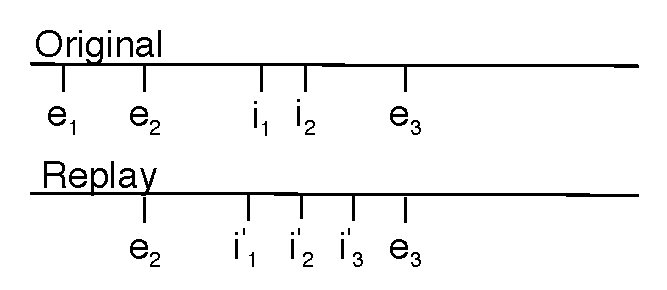
\includegraphics[width=\linewidth,height=0.8in]{../diagrams/state_machines/event_sequence.pdf}
%\end{wrapfigure}

In the general case it is always possible to construct two state machines that lead
to differing outcomes: one that only leads to the invariant violation when
we inject the next input
\emph{before} a new internal event, and another only when we inject \emph{after} a new internal
event. In other words, to be guaranteed to traverse any existing suffix that leads
to the invariant violation, we must recursively branch, trying both
possibilities for every new internal event. This implies an exponential number of
possibilities to be explored in the worst case.

Exponential search over these possibilities is not a practical option. Our heuristic when waiting for expected internal
events is to proceed normally if there are new internal events,
always injecting the next input when its last expected predecessor
either occurs or times out. This ensures that we always find suffixes that
contain a subset of the (equivalent) original internal events, but leaves open the
possibility of finding divergent suffixes that lead to the invariant
violation.
%This is reasonable because not even branching on new
%internal events is guaranteed to find the globally shortest fault-inducing input
%sequence:
%there may be other unknown
%paths through the state machine leading to the invariant violation that are
%completely disjoint from the original execution.

\eat{
Luckily, crucially ambiguous new internal events are not problematic for the
control software we evaluated, as we show in \S\ref{sec:casestudies}.
We conjecture that ambiguous new internal events are
rare because SDN software is a control plane system,
and is designed to quiesce quickly (\ie~take a small number of internal
transitions after any input event, and stop at highly connected vertices).
Concretely, SDN programs are often structured as (mostly independent) event
handlers, meaning that pruning input events simply triggers a subset of the original
event handlers.
\eat{
As an illustration, consider the state machines
in Figure~\ref{fig:state_machines}:
the controllers quickly converge to a single state (either ``Master'' or
``Backup''), as do the switches (``Safe'').
}
}

\subsection{Complexity}
\label{subsec:complexity}

The delta debugging algorithm terminates after $\Omega(\log n)$
invocations of $replay$ in the best case, and $O(n)$ in the worst case, where $n$ is the number of inputs in the original
trace~\cite{Zeller:1999:YMP:318773.318946}.
Each invocation of $replay$ takes $O(n)$ time
(one iteration for {\sc Peek()} and one iteration for the replay itself),
for an overall runtime of $\Omega(n \log n)$ best case and $O(n^2)$ worst case replayed inputs.
The runtime can be decreased by parallelizing delta debugging:
speculatively replaying subsequences in parallel, and joining the results.
Storing periodic checkpoints of the system state throughout testing can also reduce runtime, as it
allows us to replay starting from a recent checkpoint rather than the beginning of the
trace.% \barath{But doesn't this approach break due to non-determinism?  Sometimes we want
%a replay run to be different from a previous replay run...} 

\eat{
SDN platform developers can reduce the probability that the replay algorithm
will need to back up by placing causal annotations on internal
events~\cite{fonseca2007x}: with explicit causal information, the replay
algorithm can know
\apriori~whether certain internal events are dependent on pruned inputs.
}

\colin{Describe Andrew's input type pruning optimization and measurements. "We
make another optimization.."}

% In the next section we describe some of the practical challenges we have overcome to realize our approach.

% \colin{Cut this section?}
% In our initial experiments we have found that applying delta debugging to explore
% subsequences of $E_L$ and striving to maintain a single timing $T$ that maintains
% causal dependencies reliably finds small MCSes.


\section{Systems Challenges}
\label{sec:systems_challenges}
The core piece of infrastructure we need to realize our approach is a
mechanism to replay execution logs. Building such a replay mechanism comes
with many challenges; unlike the example applications described
by the original delta debugging paper~\cite{Zeller:1999:YMP:318773.318946}, the system we are troubleshooting is not a
single program--it is all the nodes and links of a distributed system,
including controllers, switches, and end-hosts. The asynchrony of distributed
systems makes it difficult to reliably replay orderings of
events without great care.

Our approach is to simulate the control-plane
behavior of network devices (with support for minimal data-plane behavior) on
a single machine. We then run the control software on
top of this simulator and connect the software switches to the controllers as if they were true
network devices, such that the controllers believe they are configuring a true
network. This setup allows the simulator to interpose on all communication
channels and delay, drop, or reorder
messages as needed. The overall
simulation architecture is depicted in
Figure~\ref{fig:architecture}.

\begin{figure}[t]
    %\hspace{-10pt}
    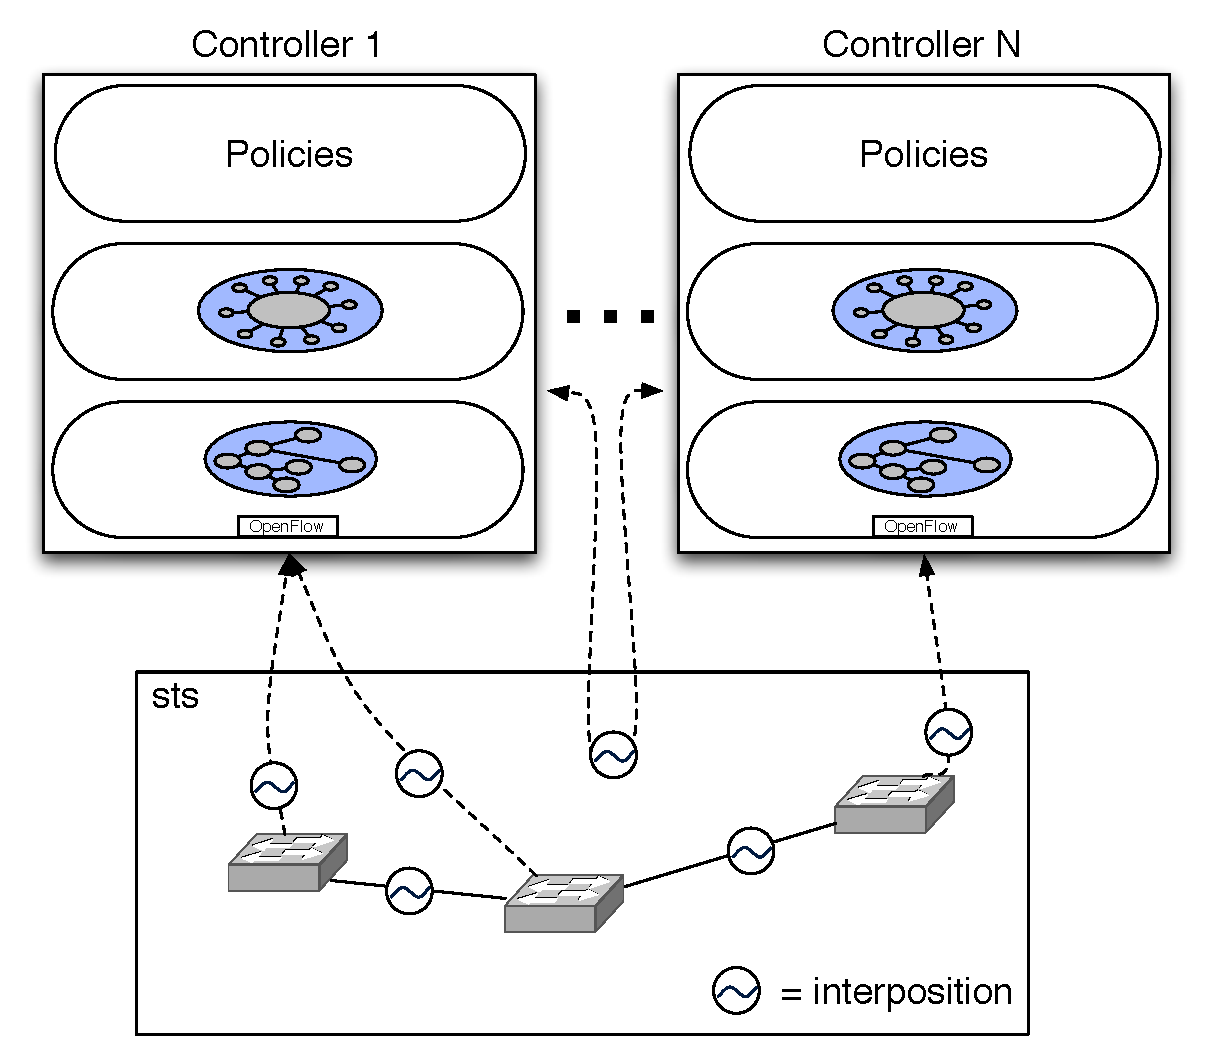
\includegraphics[width=3.25in]{../diagrams/architecture/Debugger_Architecture.pdf}
    \caption[]{\label{fig:architecture} Simulation infrastructure. We simulate
    network devices in software, and interpose on all communication
    channels.}
\end{figure}

We begin by using our simulator to perform testing on controllers to find
bugs. Our most common use case involves generating randomly chosen input
sequences~\cite{Miller:1990:ESR:96267.96279}, feeding them to controller(s),
and monitoring
invariants~\cite{hsa} at chosen intervals.
We also run the simulator interactively
so that we can examine the state of any part of the simulated network,
observe and manipulate messages, and follow our
intuition to induce orderings that they believe may trigger bugs.
In either case, controlling the inputs from a single location
allows the simulator to trivially record a global, causally-consistent
event ordering.

After discovering an invariant violation of interest, the simulator replays
the logged sequence of inputs (such as link failures, controller crashes, host migrations,
or policy changes). For example, the simulator replays link failures
by disconnecting the edge in the simulated network, and sending a
port status message from the adjacent switches to their parent controller(s).

\eat{ % Maybe add this back in? This is relatively important
The input subsequences chosen by delta debugging are not always valid. For
example, it is not sensible to replay a recovery event without a
preceding failure event; nor is it sensible to replay a host migration
event without modifying its starting position when a preceding host
migration event has been pruned. The simulator checks
validity before replaying a given subsequence to account for this
possibility.\footnote{Handling invalid inputs is crucial for
ensuring that the delta debugging algorithm we employ~\cite{Zeller:1999:YMP:318773.318946}
is guaranteed to find a minimal causal sequence, since it assumes that no unresolved
test outcomes occur. Zeller wrote a follow-on
paper~\cite{Zeller:2002:SIF:506201.506206} that removes the need for this assumption,
but incurs an additional factor of $N$ in complexity in doing so.}
Currently our simulator accounts for validity of all network state change
events (shown in Table \ref{tab:inputs}), but does not support policy changes,
which have more complex semantics.
}

\colin{Cut? 15,000 LOC systems don't jive so well with HotNet's agenda}
\projectname~(\projectmeaning) is our realization of this simulator.
\projectname~is implemented in roughly 15,000 lines of Python in
addition to the Hassel network invariant checking library~\cite{hsa}. We have
made the code
for \projectname~publicly available\footnote{Omitted to preserve anonymity.}.
To date, three industrial SDN companies have expressed interest in adopting it.

\subsection{Mitigating Non-Determinism}

We designed \projectname~to be as resilient to non-determinism as is
practically feasible, while avoiding modifications to control software whenever possible.
When sending data over multiple sockets, the operating system exhibits
non-determinism in the order it schedules the socket I/O operations.
\projectname~optionally ensures a deterministic order of messages
by multiplexing all sockets in the controller process
onto a single true socket. \projectname~currently overrides socket functionality within the control
software itself.\footnote{Only supported for POX at the moment.}
%In the future we plan to implement deterministic message ordering without code modifications by
%loading a shim layer on top of
%libc (similar to liblog~\cite{Geels:2006:RDD:1267359.1267386}).

\projectname~needs visibility into the control software's internal state
changes to reliably reproduce the system execution. We achieve this by
making a
small change to the control software's logging library\footnote{Only supported
for POX and Floodlight at the moment.}: whenever a control process executes a log
statement, we notify \projectname~that a new state transition
is about to occur, and optionally block the process. \projectname~then sends
an acknowledgment to unblock the controller after logging the state change. If blocking was enabled
during recording, we force the control software to block at internal state
transition points again during replay
until \projectname~gives explicit acknowledgment.

Routing the {\tt gettimeofday()} syscall
through \projectname~makes replay more resilient to alterations in execution
speeds.\footnote{When the pruned trace differs from the original, we make a
best-effort guess at what the return values of these calls should be. For example,
if the altered execution invokes {\tt gettimeofday()} more times than we recorded
in the initial run, we interpolate the time values of neighboring events}
%As an added benefit, overriding {\tt gettimeofday()} allows us to `compress'
%runtime in some cases (similar to time-warped emulation~\cite{Gupta06toinfinity}).

\subsection{Coping with Non-Determinism}

Our current implementation does not account for other sources of non-determinism,
such as random number generators, asynchronous signals,
or interruptable instructions (\eg~x86's block memory
instructions~\cite{Dunlap:2002:REI:844128.844148}). And even if these sources were
eliminated, it would not be possible to achieve perfectly deterministic
replay in all cases without full visibility into internal events--a daunting
instrumentation task.

Fortunately we can cope with cases of excessive non-determinism by replaying each subsequence chosen
by delta debugging multiple times. Assuming that non-determinism
is an independent and identically distributed random variable, multiple
replays yields a Bernoulli distribution $P = (1-p)^{n}$ for whether we will fail to
trigger a latent bug after $n$ replays. The Bernoulli distribution
works strongly in our favor; for example, even if the original bug is
triggered in only 20\% of replays, the probability that we will not trigger
it during an intermediate delta debugging replay is approximately
10\% if we replay 10 times per subsequence.


\section{Case Studies}
\label{sec:casestudies}
We have applied \projectname~to the routing applications\footnote{At the time
we conducted these experiments, routing was among the most complex
SDN applications publicly available. We are currently investigating
distributed controllers with more complex applications such as network virtualization,
which have recently become publicly available. We believe bugs involving
distribution are particularly amenable to techniques such as ours.} of three open
source SDN control platforms:
POX~\cite{pox}, NOX~\cite{nox}, and Floodlight~\cite{bigswitch}. We describe
bugs we found in each of these controllers to illustrate
how the minimized traces our technique produced were valuable in
understanding the bugs' root causes.

\subsection{POX In-Flight Blackhole}
After roughly 20 runs of randomly generated inputs,
we detected a persistent blackhole while
POX was bootstrapping its
discovery of link and host locations in a small 2-switch, 2-host network.
There were $29$ inputs in the initial trace, and \projectname~returned an $11$ input
MCS.

We provided the MCS to the lead developer of POX. Primarily using the
console output, we were able to trace through the code and identify the problem
within 7 minutes, and were able to find a fix for the race condition within 40
minutes. By matching the console output with the code, he found that the crucial
triggering events were two
in-flight packets (set in motion by prior traffic injection events):
POX first incorrectly learned a host location as a result of the first in-flight
packet showing up immediately after POX discovered that that port belonged to
a switch-switch link -- apparently the code had not accounted for the
possibility of in-flight packets directly following link discovery -- and
then as a result the
second in-flight packet
POX failed to return out of a nested conditional that would have
otherwise prevented the blackholed routing entries from being installed.

Although the initial trace was fairly small to begin with, knowing that every
input in the MCS was necessary for triggering the race condition allowed us to
avoid the
possibility of being mislead by extraneous diagnostic information while
tracing through the many potentially faulty code paths.

\subsection{NOX Discovery Loop}

We tested NOX on a four-node mesh, and discovered a
routing loop between three switches
within
roughly $20$ runs of randomly generated inputs.

Our initial input size was $68$ inputs, and
\projectname~returned an $18$ input MCS.\footnote{We had difficulty replaying
the final MCS. The reason seems clear: this bug depends on the
order NOX discovers links, which in turns depends on hashes computed from random memory
addresses its discovery modules LLDP selection algorithm!}
Our approach to debugging was to
reconstruct from the MCS how NOX should have installed routes, then compare
how NOX actually installed routes.

The order in which NOX discovered links was crucial: at the point NOX
installed the 3-loop, it had only discovered one link towards the destination.
Therefore all other switches had to route to the one known neighbor switch.
This comprised 2 of the 3 links involved in the link.

The destination host only sent one packet, which caused NOX to initially learn
its correct location. After NOX flooded the packet though, it became confused
about its location. One flooded packet arrived at
another switch that was currently not known to be attached to anything, so NOX
incorrectly concluded that the host had migrated. Other flooded packets were
dropped as a result of link failures in the network and randomly generated
network loss. The loop was then installed when the source injected another
packet.

This case took us roughly 10 hours to debug. We are confident that without the
minimized trace, it would have taken much
longer to trace through the subtle sequence of events that were necessary for
setting up the network in precisely the right conditions.

\subsection{Floodlight Forwarding Loop}

We applied \projectname~to Floodlight's routing application.
In about 30 minutes, our fuzzing uncovered a
117 input sequence that caused a persistent 3-node forwarding loop.
\projectname~reduced the sequence to 13 input events in 324 replays and 8.5 hours.

We repeatedly replayed the 13 event MCS, while successively adding
instrumentation and increasing the log level each run. After about 15 replay
attempts, we found that the problem was caused by interference of end-host
traffic with ongoing link discovery packets. In our experiment, floodlight had
not discovered an inter-switch link due to dropped LLDP packets, causing an
end-host to flap between perceived attachment points.

While this behavior cannot strictly be considered a bug in Floodlight,
the case-study nevertheless highlights the benefit of
\projectname~over traditional fuzzing techniques: By leveraging repeated replays
of a significantly reduced MCS, we were able to diagnose the root cause--a
complex interaction between the LinkDiscovery, Forwarding, and DeviceManager
modules.


%\section{Discussion}
%\label{sec:discussion}
%% Just realized: b/c of anonymity, the PC can't chastise us for
% running our system on our own code -- we can't tell them that it's our code!
\Simulator{} is certainly not without limitations. We discuss several of them
here.

\noindent{\bf How big is the log? How long does this take to run?}
Assuming that it takes constant time to inject an external input, the
runtime of the algorithm is $O(n^2)$, where $n$ is the number of external inputs to
prune. If the log is too long to rerun from the beginning for
every iteration, the operator can take causally-consistent
snapshots~\cite{Chandy:1985:DSD:214451.214456} of the
live system and bootstrap the simulator from the nearest quiescent snapshot.
The length of the execution can also be `compressed' by manipulating timers in the
controllers while still maintaining happens-before dependencies.

\noindent{\bf Isn't a global log difficult to obtain?} Some failure events may appear
multiple times in the log (\eg{} replica servers detecting that a master went down),
yet we only want to replay the original event.
If it is not possible to distinguish the original
failure event from the resulting events (\eg{} in the case of a disk failure
where the original crash message is not recoverable), developers may need to
manually decipher the original event.
If the simulator is unable to reproduce the correctness violation,
the simulator may be able to `fuzz' different event
orderings in an attempt to retrigger it.

\noindent{\bf Are all simulated failures really indistinguishable
from actual failures?}
Maybe not, but since the deterministic replay environment
is built in software, the fidelity of our simulated failures
can be made arbitrarily sophisticated.\footnote{subject to scalability
limitations of fine-grained simulations}

\noindent{\bf What if there are causal dependencies between inputs events?}
Developer's need to know how the
distributed system {\it reacts} to external inputs. Understanding why external
inputs occurred is an orthogonal issue.
% POSSIBLY CUT IF NOT ENOUGH SPACE
Consider a drunk network operator who (i) trips on an ethernet cable, and
consequently (ii) spills his drink on a switch (busting the hardware). Our
system views (i) and (ii) as causally independent, and that's fine, since
the developer's goal is not to debug drunk operators.

\noindent{\bf Will this approach work on all control platforms?}
\Simulator{} requires controller-specific modifications, including
awareness of the API to specify policy changes and awareness of the format of log
messages. Correspondence checking also
assumes that it has access to views with routing table-like formats.

\noindent{\bf Will control platforms ever become stable enough that
          \simulator{} is unnecessary?}
We certainly hope so! The field is decades from that point though.

%\noindent{\bf How is this specific to SDN?}
%
%Yes!

\eat{
Second, we hope to gather error logs from real production deployments which
will help us populate this repository; this may require providing novel kinds
of anonymization, so that large datacenter operators would be willing to share
their problems (since they want their SDN code to work) without revealing the
details of their network.  This may require a infrastructural counterpart to
minimally-causal events; the smallest number of infrastructure components that
can reproduce the same bug.
}

\eat{
\colin{TODO: add note about not being able to tell difference between
endogenous and exogenous events, which might hide the true cause of a bug.
This is OK though, since we assume that the platform should always have a
correct option, but it doesn't take it. That is, the root cause of the crash
is not what we're interested in (software vs. hardware), it's how the platform
reacts to that crash that matters (should be robust, no matter what the
cause of the crash)}

\andi{Don't quite know what you mean by endogenous vs. exogenous}

\colin{Note that we also assume an out-of-band management network between
switches and controllers, and that the management network always provides 
connectivity. We could add the management network into our model if we want, I
suppose.}
}

\eat{ % The production environment logs this anyway? Add this point in
      % if we have space.
\noindent{\bf Aren't the proposed production logs going to be huge?}

In contrast to general record-and-replay
mechanisms, the amount of recorded state needed for
high-fidelity replay is tractable\andi{Check with our newly, well defined strong assumptions: 
we need full internal/external events. Is this tractable}. With proactive flow installation,
updates are pushed to routing tables over a relatively long time scale; periodic
FIB snapshots along with a log of link state events, control server
downtime, host mobility information, and policy-changes suffice for our purposes.
Assuming a maximum of 256K routing or ACL entries per switch~\cite{cisco7000}, and 
36 bytes per entry, each FIB will contain a maximum of 9216
kilobytes, uncompressed. A fat tree network of 27,648 hosts
includes 2,880
switches~\cite{Al-Fares:2008:SCD:1402958.1402967}.
Therefore a snapshot of the FIBs of the entire network would naively take up roughly
26 GB. Note however, that the data is likely to be compressible quite well, due to do its
structural and temporal properties. Assuming 8.5 error events per minute per
datacenter~\cite{Greenberg:2009:VSF:1592568.1592576}, 1,000,000
VM placement changes per day per datacenter~\cite{Soundararajan:2010:CBS:1899928.1899941},
and a small rate of human-specified policy changes, the log of the external inputs
should grow at a rate of \textasciitilde 750 entries per minute.
}

%To account for host mobility, assume that each server hosts 10 VMs,
%and 1\% of VMs are created, suspended, or migrated every minute. Then 10,000 host mobility events must be
%logged per minute, also a reasonable storage cost.

\eat{
\colin{Notes from Rean Griffith:
\begin{itemize}
\item total vms in a typical datacenter: 1000
\item migration frequency (migrations/minute): 20 per hour
\item VM spin ups/downs: 150 power ons per hour (see our OSR 2010 paper for
power off estimates)
\item Do we log VM migrations and how does that log grow (I wasn't able to
get any estimates on log-growth data)
\end{itemize}

We had an OSR 2010 paper that provided numbers scaled by the number of
VMs in an installation:
Challenges in building scalable virtualized datacenter management
(http://dl.acm.org/citation.cfm?id=1899941)
}
}

%As a point of reference, border routers' working RIB size is
%$\textasciitilde$130MB~\cite{Karpilovsky:2006:UFR:1368436.1368439}.
\eat{

TODO: Replace this analysis.
It stinks. PORTLAND is not the right way to evaluate this due to the lacking number of rules.

\noindent{\bf Correspondence Checking Runtime.} 
Computing the propagation
graph for correspondence checking is equivalent to enumerating
all possible paths in the network, which scales with the diameter
of the network and the number of routing entries per switch.
The propagation graph for each host can be
computed in parallel however, so the computation is bottlenecked by the serial runtime
of computing a single host's propagation graph.

We show the serial runtime of correspondence checking in
Figure~\ref{fig:hsa_runtime}. For this analysis we generated fat tree topologies
between 2 and 48 pods wide, with pre-installed PORTLAND~\cite{NiranjanMysore:2009:PSF:1592568.1592575}
routing tables in each switch. Each data point is the minimum of three
runs on a single Intel Xeon 2.80GHz core. Note that the number of PORTLAND routing entries per switch scales with the number
of pods in the fat-tree. We excluded the time to convert
flow tables to HSA transfer functions, since transfer functions can be maintained
offline.

As the figure depicts, even for large networks
(27,648 hosts) the serial runtime of correspondence checking is reasonable for
interactive use. The number of serial tasks to be executed
is the number of hosts in the network squared, disregarding ECMP load balancing.

\begin{figure}[t]
    %\hspace{-10pt}
    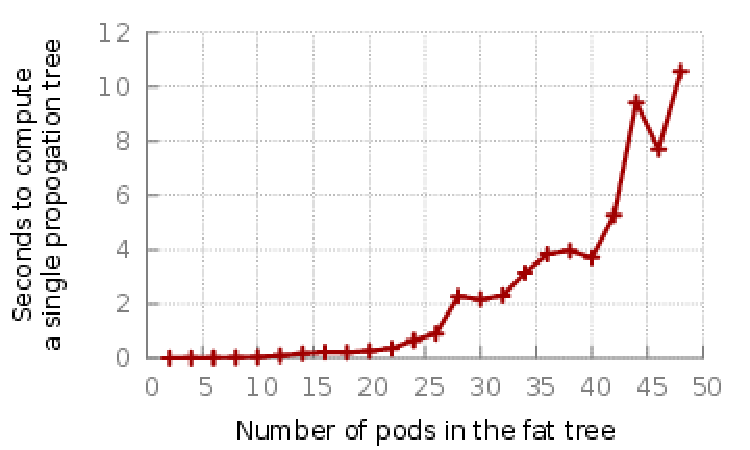
\includegraphics[width=3.25in]{../graphs/hsa_overhead_graph/graph.pdf}
    \caption[]{\label{fig:hsa_runtime} Serial runtime of correspondence
    checking on PORTLAND fat tree networks. Each datapoint consists of
    $x^3/4$ hosts and $5x^2/4$ switches (\eg{} 48 pods means 27,468 hosts
    attached to 2,880 switches)}
\end{figure}
}

\eat{ This evaluation stinks. Be gone!

\noindent{\bf Simulator Scalability.} As our approach depends on the frequently
repeating simulations, we now evaluate the setup time incurred by the simulator
system when handling large network topologies. For this experiment, shown in
Figure~\ref{fig:scalability}, we generate fat tree topologies between 2 and 48
pods wide, where all switches in the network connected to a single controller.
The controller sends each switch an OpenFlow $FLOW\_MOD$ and subsequent
$BARRIER\_REQUEST$ message, and waits for the corresponding $BARRIER\_REPLY$. We
then measure the time to between the first $FLOW\_MOD$ sent and the last
$BARRIER\_REPLY$ received. As expected, the runtime was roughly linear with the
number of switches in the network. The figure also shows that the processing
time for large networks (5 seconds per simulator round) was well within the
bounds for interactive use.

\begin{figure}[t]
    %\hspace{-10pt}
    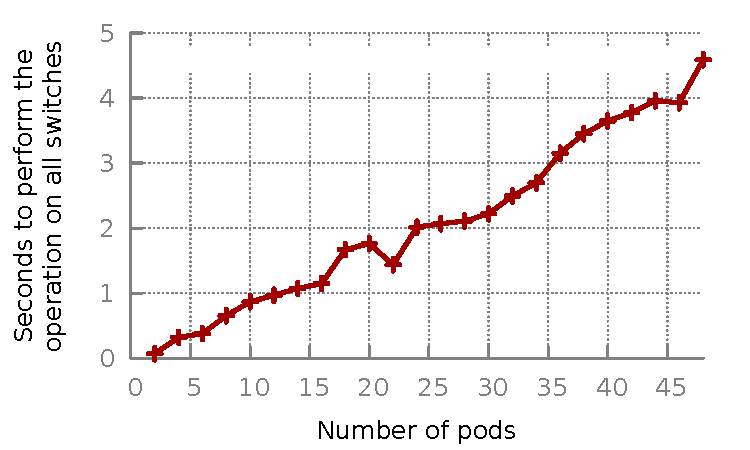
\includegraphics[width=3.25in]{../graphs/scalability_graph/scale.pdf}
    \caption[]{\label{fig:scalability} Time to send and process messages
    between controller and simulated switches. Each datapoint consists of
    $x^3/4$ hosts and $5x^2/4$ switches (\eg{} 48 pods means 27,468 hosts
    attached to 2,880 switches)}
\end{figure}

We also tested the extreme limits of the simulator's scalability, pushing up
the number of switches until something broke. We encountered what appears to be
a limitation of the Linux TCP/IP stack: TCP connection attempts began failing
beyond 26,680 sockets. Note that 26,680 switches is an order-of-magnitude larger than
the today's biggest networks.
}


\section{Related Work}
\label{sec:related_work}
%-- Program Slicing --

The delta debugging algorithm~\cite{Zeller:2002:SIF:506201.506206} seeks to solve
a problem that is exactly analogous to ours on a single machine: given input that causes a test case
to fail, what is the minimum subset of the input that still produces the failure?
We apply the same reasoning to a distributed system.

%-- Deterministic Replay (OFRewind) --

Deterministic replay techniques such as OFRewind~\cite{ofrewind}
are designed to allow developers to interactively prune
the inputs that lead up to errant behavior. We present an algorithm that
automates this process.

%-- Model checking (NICE): --

NICE~\cite{nice} combines model checking with concolic execution
to enumerate all possible code paths taken by control software (NOX)
and identify concrete inputs (\eg{} control message orderings) that cause
the network to enter invalid configurations. Unlike NICE, by analyzing
bugs {\em post-hoc} from live runs of the system our approach applies
to large software systems without suffering from state explosion.

%-- Invariant Checking? --

\eat{
Invariant checking tools such as Anteater~\cite{anteater} and HSA~\cite{hsa}
detect problems in the dataplane. We leverage invariant checking tools
to distinguish inputs that are necessary for reproducing a given invariant violation.
}

%-- Root cause analysis? --

Root cause analysis techniques~\cite{577079} seek to identify the minimum set of failed
components (\eg{} link failures) needed to explain a collection of alarms. Rather than
focusing on individual component failures, we seek to minimize inputs that affect the behavior
of the overall distributed system.

%-- Distributed Systems debuggers --

Pip~\cite{pip} is a framework for instrumenting general-purpose distributed systems
with code to record, display, and check invariants on causal paths throughout
live executions. \Simulator{} observes the causal behavior of the
distributed system in a simulated environment, enabling us to iteratively prune extraneous input events.

%-- Simulators? --
%
%Several other network simulators exist for testing SDN controllers. Mininet is a
%platform for emulating OpenFlow switches and hosts within a single
% VM~\cite{Lantz:2010:NLR:1868447.1868466}. The ns-series of network simulators
%provides a general framework for testing new protocols, topologies,
%and traffic mixes~\cite{ns3}. We found that these existing simulators did
%not provide sufficient support for the corner-cases situations which are the
%focus of our work, such as failures and VM migration.

%-- Distributed Systems --
%
%Many of our ideas originate from the literature on troubleshooting general
%distributed systems. WiDS checker introduced the notion of recording
%production executions to be later replayed and verified in a controlled simulation.
% Finally, end-to-end tracing
%frameworks such as X-Trace~\cite{Fonseca:2007:XPN:1973430.1973450} and
%Pinpoint~\cite{Chen02pinpoint:problem} provide a framework for tracing requests throughout
%a distributed system in order to infer correctness errors between layers and
%across components. Our work solves a more constrained problem; we leverage
%the structure of the SDN stack to enable a simple notion of platform
%correctness. In addition, these systems assume that invariants should hold at
%all times; we observe that in an eventually-consistent system such as SDN,
%transient policy-violations are inevitable. We built \simulator{} to help troubleshooters
%differentiate ephemeral from persistent errors.

% If we manage to run multiple applications by Monday, we should cite papers
% on consistency and cross-layer debugging:
%X-Trace~\cite{xtrace}
% Vector Clocks
% Onix
% Virtualization definitely won't happen by Monday. But, papers include
% Martin's presto '10 paper 'Virtualizaing the Network Forwarding Plane'



\section{Conclusion}
\label{sec:conclusion}
\colin{Insight to add: testing/simulation is the *main* value proposition of
SDN for Google. It is *the* main reason they have adopted it}

SDN's purpose is to make networks easier to manage. SDN
does this, however, by pushing complexity into SDN control software itself. Just
as sophisticated compilers are hard to write, but make programming easy, SDN
control software makes network management easier, but only by forcing the
developers of SDN control software to confront the challenges of asynchrony,
partial failure, and other notoriously hard problems inherent to all distributed
systems.
%Thus, people will be troubleshooting and debugging SDN control software for many
%years to come, until it becomes as stable as compilers are now.

Current techniques for troubleshooting SDN control software are primitive; they
essentially involve manual inspection of logs in the hope of identifying the
triggering inputs. Here we developed a technique for automatically
identifying a minimal sequence of inputs responsible for triggering a given
bug, without making assumptions about the language or instrumentation of the
software. We believe our technique will be especially valuable for troubleshooting
distributed controllers running complex applications, which are just now
becoming publicly available.

We focused on SDN control software, but we believe our techniques
are applicable to general distributed systems. As distributed systems
proliferate, we hope that our technique helps ameliorate the dearth of
tools in this important area.\\[0.2ex]

%We have applied this system to three open source SDN platforms.
%Of the five bugs we encountered in a five day investigation,
%our technique reduced the size of the trace to 2 inputs in the best
%case and 18 inputs in the worst case.

\eat{
SDN is widely heralded as the ``future of networking'', and its purpose is to make
it easy to manage networks. Achieving this end forces platform developers to directly
confront asynchrony, partial failure, and other problems that are inherent to all distributed
systems and notoriously difficult to get right.

In this paper we developed a technique for automatically
identifying a minimal sequence of inputs responsible for triggering a given bug.
We have applied this system to three open source SDN platforms, and
were able to find or reproduce bugs in all the platforms we investigated.
%Now we just need to provide a mechanism for the next question: would that date
%have panned out if I hadn't spilt the wine?
}

% Two ideas that have been put on the backburner:
% - distinguishing persistent violations from transient
% - using correspondence checking to localize the layer where the bug first
%   manifests

%We chose SDN as our domain becuase X,Y,Z. We envision a new paradigm where
%domain knowledge is applied to debugging in all systems.

% ------------------------------------------- %
%             OLD TEXT
\eat{
It does so by moving control plane functionality out of
network devices, and into a tightly-coupled cluster of servers that provide a simple
programmatic interface through which policies can be specified. As we have
learned in this work, the challenges of maintaining virtualized and distributed
views in a failure-prone environment are
notably different from the challenges encountered in traditional,
fully distributed control planes.

}


\bibliographystyle{abbrv} \small \bibliography{bib}

%\input{appendix}

\end{document}
